\documentclass[times, utf8, seminar]{fer}
\usepackage{booktabs}
\usepackage{booktabs}
\usepackage{pdfpages}
\usepackage{braket}
\usepackage[inkscapeformat=png]{svg}
\usepackage{subcaption}
\usepackage[qm]{qcircuit}
\usepackage{graphicx}
\usepackage[noend]{algpseudocode}
\usepackage{algorithm}
\usepackage{amsmath}
\usepackage{amssymb}
\usepackage{listings}
\usepackage{makecell}
\usepackage{tabularx}
\usepackage{cellspace}
\usepackage{graphicx}
\usepackage{array, tabularx, caption, boldline}
\usepackage{framed}

\usepackage{courier}
\usepackage{url}
\usepackage[pdfa, hidelinks]{hyperref}

\def\UrlBreaks{\do\/\do-}
\setcitestyle{numbers,square,super}
\hypersetup{
	citecolor=black
}
\newfloat{Kod}
\captionsetup{Kod}

\newfloat{Ispis}
\captionsetup{Ispis}

\begin{document}
	
	% TODO: Navedite naslov rada.
	\title{Algoritam šišmiša i algoritam kukavičjeg pretraživanja}
	
	% TODO: Navedite svoje ime i prezime.
	\author{Velimir Kovačić}
	
	% TODO: Navedite ime i prezime mentora.
	\voditelj{Marin Golub}
	
	\maketitle
	
	\tableofcontents
	
	\chapter{Uvod}
	\hspace{\parindent} Metaheuristika se odnosi na oblikovni obrazac ugrađivanja prethodno stečenog znanja u izgradnju optimizacijskih algoritama. Smatra se potpodručjem stohastičke optimizacije. Stohastička optimizacija je kombinacija algoritama i slučajnih procesa radi pronalaženja optimalnih rješenja. 

Prirodom nadahnute metaheuristike su one koje crpe ideje za pretraživanje prostora stanja iz prirode. Algoritmi rojeva su potkategorija prirodom nadahnutih metaheuristika. Svoja svojstva crpe iz kolektivnog ponašanja životinja i kukaca. Roj se sastoji od više individua čije je ponašanje vrlo jednostavno, ali zajedno mogu djelovati inteligentno. Postoje mnogi takvi algoritmi, najpoznatiji su mravlji algoritam i algoritam pčela. 

U ovom seminaru razmatraju se manje poznati algoritmi: algoritam šišmiša i algoritam kukavičjeg pretraživanja. Oba su algoritma opisana i prikazan je njihov pseudokod. Navedeni su načini na koje se algoritmi mogu lokalno pokrenuti i dani su primjeri raznih primjena algoritama. 

	\chapter{Algoritam šišmiša}
	\section{Uvod}
\hspace{\parindent}Algoritam šišmiša\cite{Yang2010} (BA) metaheuristički je optimizacijski algoritam iz skupine algoritama rojeva čestica. Nadahnut je eholokacijom šišmiša. 

\hspace{\parindent} Šišmiši su sisavci iz roda \textit{Chiroptera} i ujedno jedini sisavci s krilima. Tvore oko 20\% svih vrsta sisavaca.  Dijele su 2 podreda: veliki šišmiši (\textit{Macrochiroptera}) i mali šišmiši (\textit{Microchiroptera}). Iako sve vrste koriste eholokaciju u nekoj mjeri,  šišmiši iz reda malih šišmiša je koriste opsežnije.\cite{netopiri}  Eholokacija kod malih šišmiša oblik je sonara, odašilju vrlo glasan i kratkotrajan zvučni impuls te primaju jeku koju je izazvao odbijajući se od okoline. Služi im za pronalaženje plijena, svojih legla i izbjegavanje prepreka u mraku. 

\hspace{\parindent} Za većinu vrsta impuls traje između 5 i 20 ms i ima konstantnu frekvenciju u intervalu od 25 kHz do 150 kHz. U normalnim uvjetima taj impuls odašilju 10 do 20 puta u sekundi, dok  ga prilikom lova mogu odašiljati i do 200 puta u sekundi. Ispostavlja se da šišmiši imaju izrazitu sposobnost obrade signala. Uz pretpostavku brzine zvuka od 340 m/s, može se odrediti da je valna duljina impulsa između 2mm i 14mm za frekvencijski raspon od 25 kHz do 150 kHz. Intenzitet zvuka može biti do 110 dB, a smanjuje se što je šišmiš bliže plijenu.

\section{Algoritam}
\hspace{\parindent}U samom algoritmu potrebno je idealizirati svojstva eholokacije:
\begin{enumerate}
	\item Svi šišmiši koriste eholokaciju radi određivanja udaljenosti.
        \item Znaju razliku između plijena i prepreka.
	\item i-ti šišmiš leti brzinom $\vec{v_i}$, na položaju $\vec{x_i}$, s frekvencijom $f_i$ i intenzitetom zvuka $A_i$.
 \item Šišmiši namještaju frekvenciju zvučnih impulsa i učestalost odašiljanja $r \in [0,1]$ prema udaljenosti od plijena.
	\item Intenzitet zvuka je u intervalu $[A_{\text{min}}, A_0]$.
 \item Frekvencija je u intervalu $[f_{\text{min}},f_{\text{max}}]$.
\end{enumerate}


Pretpostavlja se da postoji $N$ šišmiša u prostoru dimenzije $n$. U svakoj iteraciji algoritma, svaki šišmiš izvodi 3 radnje:
\begin{enumerate}
    \item Kretanje
    \item Lokalna pretraga
    \item Ažuriranje intenziteta zvuka i učestalosti odašiljanja
\end{enumerate}





\subsection{Kretanje}
\hspace{\parindent}Kretanje je slično kretanju čestica u algoritmu roja čestica. U svakom koraku vektor brzine se usmjeri prema najboljem rješenju i odvije se kretanje šišmiša. Promjena vektora brzine ovisi o frekvenciji. 

Položaj $i$-tog od $N$ šišmiša u koraku $t$ predstavlja $n$-dimenzionalni vektor:
\begin{equation}
	\vec{x_i}^t = (x_{i1}^t, x_{i2}^t, \dots, x_{in}^t)
\end{equation}
Brzinu $i$-tog od $N$ šišmiša u koraku $t$ predstavlja $n$-dimenzionalni vektor:
\begin{equation}
	\vec{v_i}^t = (v_{i1}^t, v_{i2}^t, \dots, v_{in}^t)
\end{equation}
U koraku $t$ računa se nova frekvencija:
\begin{equation}
	f_i = f_{\text{min}} + (f_{\text{max}} - f_{\text{min}})\beta
\end{equation}

gdje je $\beta$ realan broj uzorkovan iz uniformne razdiobe na intervalu $[0,1]$.\\
U koraku $t$ računa se nova brzina:
\begin{equation}
	\vec{v_i}^t = \vec{v_i}^{t-1} + (\vec{x_i}^* - \vec{x_i}^{t-1})f_i
\end{equation}

gdje je $\vec{x_i}^*$ položaj šišmiša s najvećom vrijednošću ciljne funkcije u koraku $t-1$.\\
U koraku $t$ računa se novi položaj:
\begin{equation}
	\vec{x_i}^t = \vec{x_i}^{t-1} + \vec{v_i}^{t}
\end{equation}

\subsection{Lokalna pretraga}
\hspace{\parindent}Nakon što su svi šišmiši završili s kretanjem, pokreće se lokalna pretraga za svakog šišmiša. Lokalna je pretraga nasumična. Položaj šišmiša se ažurira na sljedeći način:
\begin{equation}
	\vec{x}_\text{novi} = \vec{x}_\text{stari} + \varepsilon A^t
\end{equation}
gdje je $\varepsilon$ slučajan broj iz intervala $[-1, 1]$, a $A^t$ je srednja vrijednost intenziteta zvuka svih šišmiša.


\subsection{Intenzitet zvuka i učestalost odašiljanja}
\hspace{\parindent}Ako je iznos funkcije cilja u novom položaju šišmiša bolji od onog u prethodnom, novi se  položaj prihvaća te se ažuriraju intenzitet zvuka i učestalost odašiljanja.
U koraku $t$ računa se novi intenzitet zvuka:
\begin{equation}
	A_i^{t} = \alpha A_i^{t - 1}
\end{equation}
U koraku $t$ računa se nova učestalost odašiljanja:
\begin{equation}
	r_i^{t} = r_i^{0}[1 - e^{-\gamma(t-1)}]
\end{equation}
Konstante $\gamma$ i $\alpha$ su parametri algoritma. Oni određuju brzinu konvergencije. Za svaki $ 0 < \alpha < 1$ i $\gamma > 0$, vrijedi:
\begin{equation}
	\lim_{t \to \infty} A_i^{t} = 0
\end{equation}
\begin{equation}
	\lim_{t \to \infty} r_i^{t} = r_i^{0}
\end{equation}
Za $r_i = 1$ i $A_i = 0$, algoritam degradira u obični algoritam roja čestica.






\subsection{Pseudokod}

\begin{algorithm}[H]
	\begin{algorithmic}[1]
		\Function{BA}{obj(x), n, N, fmin, fmax, Amin, A0, maxIter, $\alpha$, $\gamma$}
		
\State x = \Call{InitX}{n, d}

\State v = \Call{InitV}{n, d}

\State f = \Call{InitF}{fmin, fmax}
  
\State A = \Call{InitA}{Amin, A0}
  
  \State r0 = r = \Call{InitR}{0,1} \Comment{Inicijalizacija struktura podataka}

  
  \For{iter = 1 to maxIter}
		\For{i = 1 to N} 
  
                
                \State b = \Call{UniformDist}{0, 1}
                \State f[i] = fmin + (fmax - fmin)*b
                \State v'[i] = v[i] + (x* - x[i]) * f[i]
                \State x'[i] = x[i] + v[i] \Comment{Kretanje šišmiša}

                \State rand = \Call{UniformDist}{0, 1}
                \If{rand > r[i]}
                \State x'[i] = x* + \Call{NormalDistVec}{n, 0, 1}
                \EndIf
                \State e = \Call{UniformDistVec}{n, -1, 1}
                \State Amean = \Call{Mean}{A} 
                \State x'[i] = x'[i] + Amean*e \Comment{Lokalna pretraga}
                \State rand = \Call{UniformDist}{0, 1}
                \If{rand < A[i] AND obj(x'[i]) < obj(x[i])}
                    \State x[i] = x'[i] \Comment{Prihvat novog rješenja}
                    \State v[i] = v'[i]
                    \State A[i] = $\alpha$ * A[i]
                    \State r[i] = r0[i] * (1 - e**(-$\gamma$ * iter))
                \EndIf
                \EndFor
		\State x* = \Call{MaxArg}{obj(x)}
		\EndFor
		\State \Return x*	
		\EndFunction
	\end{algorithmic}
	\caption{Algoritam šišmiša}
\end{algorithm}







\section{Programsko ostvarenje}
\subsection{Primjer funkcije za minimizaciju}
Neka se minimizira $n$-dimenzionalna funkcija:
\begin{equation}
    f(\vec{x}) = \sum_{i = 1}^{n}x_i^2 + 25\sum_{i = 1}^{n}\sin^2{x_i} \label{eq:fx}
\end{equation}



\begin{figure}[H]
	\centering
	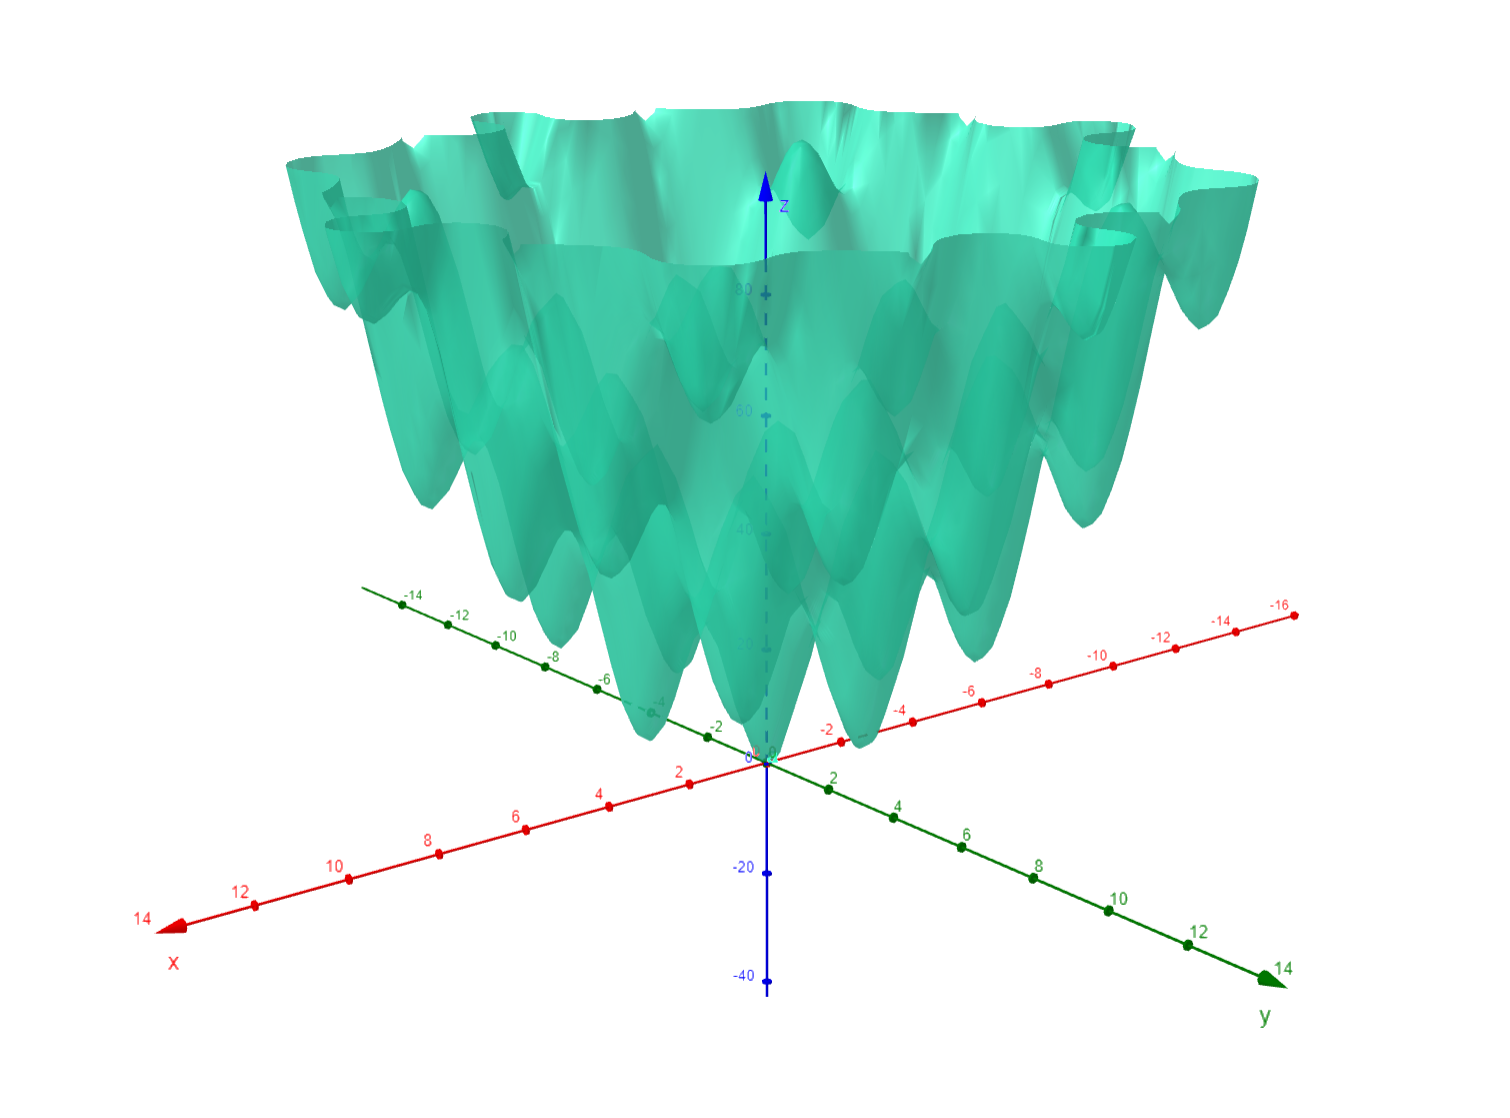
\includegraphics[width=14cm]{eggcrate_func.png}
	\caption{Graf funkcije $f(\vec{x})$ za $n = 2$} 
\end{figure}

Funkcija ima minimum u točki $\vec{0}$ i on iznosi $f(\vec{0}) = 0$. 


\subsection{Programsko ostvarenje MEALPY} \label{MP:Bat}
\hspace{\parindent}Algoritam šišmiša i mnogi drugi metaheuristički algoritmi programski su ostvareni u sklopu knjižnice programa otvorenog koda MEALPY\cite{van2023mealpy} programskog jezika Python. Knjižnica se može preuzeti naredbom konzole:

\begin{figure}[H]
	\begin{framed}
		\begin{footnotesize}
			\begin{verbatim}
		> pip install mealpy\end{verbatim}
		\end{footnotesize}
	\end{framed}
	\captionof{Kod}{Naredba konzole za preuzimanje knjižnice MEALPY}
\end{figure}

\hspace{\parindent}Prethodno opisani problem funkcije \eqref{eq:fx} s $n = 10$ definira se u programu kao rječnik i pokreće se algoritam šišmiša s 1000 iteracija, brojem šišmiša $N = 50$,  $\alpha = \gamma = 0.9$, $[A_{\text{min}}, A_0] = [1, 2]$,  $[f_{\text{min}}, f_{\text{max}}] = [-10, 10]$. U razredu \verb|BA| postoji više različitih inačica algoritma, najsličniji opisanom je \verb|AdaptiveBA|, stoga je on korišten u primjeru.

\begin{figure}[H]
	\begin{framed}
		\begin{footnotesize}
			\begin{verbatim}
import numpy as np
from mealpy import FloatVar, BA
from numpy import pi as PI

n = 10

def objective_function(solution):
    return np.sum(solution**2) + 25*np.sum(np.sin(solution)**2)

problem = {
    "obj_func": objective_function,
    "bounds": FloatVar(lb=(-2*PI,)*n, ub=(2*PI,)*n),
    "minmax": "min",
}


model = BA.AdaptiveBA(epoch=1000, pop_size=50, 
                      loudness_min = 1.0, loudness_max = 2.0,
                      pf_min = -10., pf_max = 10.)

g_best = model.solve(problem)

print("Solution:", g_best.solution)
print("Fitness:", g_best.target.fitness)
			\end{verbatim}
		\end{footnotesize}
	\end{framed}
	\captionof{Kod}{Pokretanje optimizacije vlastite funkcije}
\end{figure}

\begin{figure}[H]
	\begin{framed}
		\begin{footnotesize}
			\begin{verbatim}
Solution: [-0.07566663 -2.81959093 ...  0.12792114]
Fitness: 106.61031296676825
			\end{verbatim}
		\end{footnotesize}
	\end{framed}
	\captionof{Ispis}{Ispis primjera}
\end{figure}





\section{Algoritam šišmiša u primjeni}

\subsection{Modeliranje dinamike bioloških sustava}
\hspace{\parindent}Algoritam šišmiša korišten je za prilagodljiv odabir vrijednosti parametara modela za rekonstrukciju dinamike bioloških sustava.\cite{lin2012} Uspješnost metode je pokazana na primjeru procjene parametara dinamike endocitoze.



\subsection{Procjena položaja ljudskog tijela}
\hspace{\parindent} Praćenje položaja ljudskoj tijela iz snimaka u laboratorijskim uvjetima postavljeno je kao 31-dimenzionalni optimizacijski problem.\cite{akhtar2012} Pokazano je da algoritam šišmiša radi bolje od drugih srodnih algoritama (poput algoritma roja čestica.)



\subsection{Grupiranje}
\hspace{\parindent} Razvijen je algoritam grupiranja temeljen na algoritmu K-sredina i algoritmu šišmiša.\cite{komarasamy2012} Algoritam ne zahtijeva definiranje hiperparametra K, nego sredine pronalazi korištenjem algoritma šišmiša. Prednost je ubrzanje brzine konvergencije algoritma šišmiša i smanjivanje ovisnosti algoritma K-sredina o početno odabranim sredinama.

\subsection{Problem ekonomske raspodjele opterećenja}
\hspace{\parindent} U problemu ekonomske raspodjele opterećenja, cilj je zadovoljiti potrebe za energijom uz minimalne financijske troškove. Optimizacija termalne elektrane provedena je algoritmom šišmiša uz rezultate bolje od rezultata drugih srodnih algoritama.\cite{biswal2013}

\subsection{Podudaranje slika}
\hspace{\parindent} Problem podudaranja slika u računalnom vidu je poistovjećivanje slika istih objekata slikanih u različitim uvjetima.\cite{zhangjia2012} Algoritam šišmiša, uz dodatak mutacija, korišten je za rješavanje ovog problema. Pokazano je da je takav algoritam na ovom problemu učinkovitiji od običnog algoritma šišmiša.

\subsection{Odabir značajki}
\hspace{\parindent} Binarna inačica algoritma šišmiša korištena je za odabir optimalnog podskupa značajki.\cite{6382769} Pristup spaja istraživačku moć šišmiša i brzinu klasifikatora \textit{Optimum-Path Forest} za maksimizaciju točnosti na skupu za provjeru. Pokusima je utvrđeno da takav pristup ima bolje performanse od drugih poznatih algoritama.

\subsection{Optimizacija sustava rezervoara}
\hspace{\parindent} Algoritam šišmiša upotrebljen je za optimizaciju rezervoarskog sustava Karoun-4 u Iranu.\cite{doi:10.1061/(ASCE)WR.1943-5452.0000498} Algoritam je bio učinkovitiji od linearnog programiranja, nelinearnog programiranja i genetskog algoritma. 

\subsection{Online učenje unaprijednih neuronskih mreža}
\hspace{\parindent} Online učenje slojeva unaprijednih neuronskih mreža provedeno je algoritmima: BA, GA i PSO.\cite{khankoffka2012} Usporednom analizom bilo je vidljivo da algoritam šišmiša ima bolje performanse od ostalih.
	
	\chapter{Algoritam kukavičjeg pretraživanja}
	
\section{Uvod}
\hspace{\parindent} Algoritam kukavičjeg pretraživanja \cite{gandomi2013}  (CSA) metaheuristički je optimizacijski algoritam utemeljen na parazitskom ponašanju nekih vrsta kukavica i slučajnoj šetnji (L\'evyjevom letu.) 



\subsection{Kukavičji parazitizam}
\hspace{\parindent}Kukavice su ptice iz porodice \textit{Cuculidae}, jedine porodice u redu \textit{Cuculiformes}. Mnoge vrste kukavica nesu jaja u gnijezda drugih ptica. To ponašanje se naziva \textit{parazitiranje legla}.  Neke vrste kukavica evoluirale su tako da im jaja veličinom i bojama sliče jajima vrste domaćina. Time je vjerojatnost da će ptica domaćin izbaciti njihova jaja manja, a reproduktivna moć samih kukavica veća. Uz to, kukavice se liježu ranije i instinktivno izbacuju ostala jaja iz gnijezda, povećavajući si vjerojatnost opstanka.

\subsection{L\'evyjev let}
\hspace{\parindent}U prirodi, životinje traže hranu na slučajan ili kvazi-slučajan način. L\'evyjev let je slučajna šetnja u kojoj je duljina koraka iz L\'evyjeve razdiobe ili neke druge stabilne razdiobe. Razdioba je stabilna ako je linearna kombinacija dvije nezavisne jednako distribuirane slučajne varijable, koje prate tu razdiobu, također prati tu razdiobu do na parametre. Funkcija gustoće L\'evyjeve razdiobe je:

\begin{equation}
    f(x;\mu, c) = \sqrt{\frac{c}{2\pi}}\frac{e^{-\frac{c}{2(x-\mu)}}}{(x-\mu)^{\frac{3}{2}}}
\end{equation}

gdje je $\mu$ parametar lokacije, a $c$ parametar skaliranja. Za $c = 1$ i $\mu = 0$ (bez skaliranja i pomaka), funkcija gustoće je:

\begin{equation}
    f(x) = \frac{1}{\sqrt{2\pi}}\frac{e^{-\frac{1}{2x}}}{x^{\frac{3}{2}}}
\end{equation}

\begin{figure}[H]
	\centering
	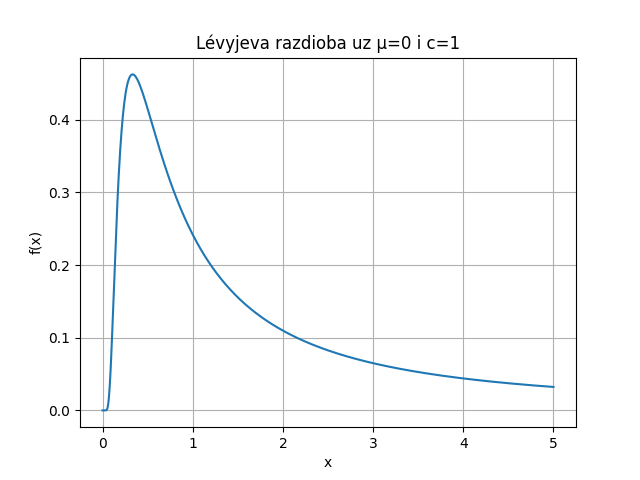
\includegraphics[width=14cm]{levy_dist.png}
	\caption{Graf L\'evyjeve razdiobe za $\mu = 0$ i $c = 1$} 
\end{figure}

Radi jednostavnosti, za određivanje duljine koraka $s$ u L\'evyjevom letu, koristi se sljedeća stabilna razdioba:

\begin{equation}
    L(s) \sim |s|^{-1 - \beta}
\end{equation}
gdje je parametar $\beta \in \langle0, 2]$. Prije upotrebe tu je razdiobu potrebno skalirati.

\begin{figure}[H]
	\centering
	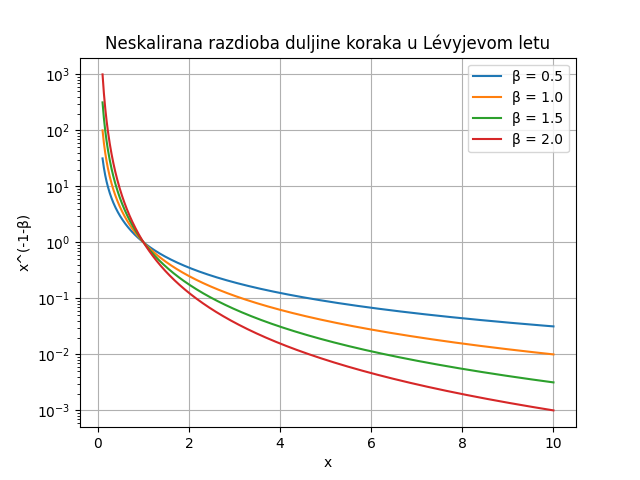
\includegraphics[width=14cm]{levy_step.png}
	\caption{Graf neskalirane razdiobe za L\'evyjev let na logaritamskoj skali} 
\end{figure}


\section{Algoritam}
U samom algoritmu potrebno je idealizirati ponašanje kukavica:
\begin{enumerate}
	\item Kukavice liježu po jedno jaje u nasumično odabrano gnijezdo.
        \item Gnijezda s dobrim jajima (rješenjima) prenose se na sljedeću generaciju.
	\item Broj domaćina je fiksan.
        \item Domaćin može otkriti strano jaje s vjerojatnošću $P_a$.
        \item Ako domaćin otkrije strano jaje, izbacuje ga ili gradi novo gnijezdo na drugoj lokaciji.
\end{enumerate}

Pretpostavlja se $N$ kukavičjih gnijezda u prostoru dimenzije $n$. U svakoj iteraciji algoritma, slučajno odabrana kukavica izvodi 2 radnje:
\begin{enumerate}
    \item Izlegne se i nasumično leti (izvodi L\'evyjev let)
    \item Zamjenjuje slučajno odabrano gnijezdo, ako je na njenom položaju vrijednost funkcije cilja veća
\end{enumerate}

Nakon što se $N$ puta odabere slučajna kukavica, udio od $Pa$ najlošijih gnijezda se izbacuje. Točnije, modificiraju se L\'evyjevim letovima.


\subsection{Kretanje}
Položaj $i$-tu od $N$ kukavica u koraku $t$ predstavlja $n$-dimenzionalni vektor:
\begin{equation}
	\vec{x_i}^t = (x_{i1}^t, x_{i2}^t, \dots, x_{in}^t)
\end{equation}
L\'evyjev let za $i$-tu od $N$ kukavica u koraku $t$ odvija se na sljedeći način:
\begin{equation}
    \vec{x}_i^{t+1} = \vec{x}_i^{t} + \alpha \oplus L(\beta)
\end{equation}
gdje je $\alpha$ faktor skaliranja, a operator $\oplus$ predstavlja međusobno množenje pripadnih elemenata vektora.


\subsection{Pseudokod}


\begin{algorithm}[H]
	\begin{algorithmic}[1]
		\Function{CSA}{obj(x), n, N, Pa, $\alpha$, $\beta$, maxIter}
		
\State x = \Call{InitX}{n, d} \Comment{Inicijalizacija struktura podataka}

  
  \For{iter = 1 to maxIter}

    \For{k = 1 to N}
    \State i = \Call{RandInt}{0, N} \Comment{Slučajan odabir kukavice}
    \State x[i] = x[i] + $\alpha \oplus L(\beta)$  \Comment{L\'evyjev let}
    \State j = \Call{RandInt}{0, N} \Comment{Slučajan odabir gnijezda}
    \If{obj(x[i]) > obj(x[j])}
        \State x[j] = x[i] 
    \EndIf
    \EndFor

    
    \State x = \Call{SortBy}{x, obj}   \Comment{Uzlazno sortiranje po funkciji cilja}
    \For{i = 1 to Pa*N} 
        \State x[i] = x[i] + $\alpha \oplus L(\beta)$ \Comment{Najlošija gnijezda se "izbacuju"}
    \EndFor
    \State x* = \Call{MaxArg}{obj(x)}
  \EndFor
		\State \Return x*	
		\EndFunction
	\end{algorithmic}
	\caption{Algoritam kukavičjeg pretraživanja}
\end{algorithm}









\section{Programsko ostvarenje}

\subsection{Programsko ostvarenje MEALPY}
\hspace{\parindent}Algoritam kukavičjeg pretraživanja ostvaren je u sklopu knjižnice programa otvorenog koda MEALPY\cite{van2023mealpy} programskog jezika Python. Knjižnica je detaljnije opisana u pododjeljku \ref{MP:Bat}.

\hspace{\parindent}Prethodno opisani problem funkcije \eqref{eq:fx} s $n = 10$ definira se u programu kao rječnik i pokreće se algoritam kukavičjeg pretraživanja s 1000 iteracija, brojem šišmiša $N = 50$ i vjerojatnošću otkrivanja $P_a = 0.3$.

\begin{figure}[H]
	\begin{framed}
		\begin{footnotesize}
			\begin{verbatim}
import numpy as np
from mealpy import FloatVar, CSA
from numpy import pi as PI

n = 10

def objective_function(solution):
    return np.sum(solution**2) + 25*np.sum(np.sin(solution)**2)

problem = {
    "obj_func": objective_function,
    "bounds": FloatVar(lb=(-2*PI,)*n, ub=(2*PI,)*n),
    "minmax": "min",
}

model = CSA.OriginalCSA(epoch=1000, pop_size=50, p_a = 0.3)

g_best = model.solve(problem)

print("Solution:", g_best.solution)
print("Fitness:", g_best.target.fitness)			\end{verbatim}
		\end{footnotesize}
	\end{framed}
	\captionof{Kod}{Pokretanje optimizacije vlastite funkcije}
\end{figure}

\begin{figure}[H]
	\begin{framed}
		\begin{footnotesize}
			\begin{verbatim}
Solution: [-0.12270494 -0.92564155 ...  2.82223478]
Fitness: 73.53109251662303
			\end{verbatim}
		\end{footnotesize}
	\end{framed}
	\captionof{Ispis}{Ispis primjera}
\end{figure}



\section{Algoritam kukavičjeg pretraživanja u primjeni}

\subsection{Optimizacija strukture automobilskih dijelova}
\hspace{\parindent} Algoritam kukavičjeg pretraživanja primijenjen je na problem problem optimizacije strukturnog dizajna automobilskih dijelova.\cite{durgun2012} Pokazano je da algoritam pronalazi dobra rješenja. 

\subsection{Pronalazak rubova slika}
\hspace{\parindent} Algoritam je upotrebljen za optimizaciju parametara antecedensa za sustav za pronalaženje rubova utemeljen na Sobelovoj tehnici i neizrazitim intervalima.\cite{7256924} Problem je složen zbog uporabe neizrazitih intervala, stoga se koriste heurističke metode. Zaključeno je da je algoritam kukavičjeg pretraživanja učinkovit za ovakve probleme.

\subsection{Pronalazak štete na mostovima}
\hspace{\parindent} Pronalazak štete na mostovima i gredama problem je koji se rješavao umjetnim neuronskim mrežama.\cite{TRANNGOC2019109637} Učenje težina neuronske mreže algoritmom kukavičjeg pretraživanja bilo je brže i točnije od učenja evolucijskim algoritmom.

\subsection{Modeliranje toka goriva zrakoplova}
\hspace{\parindent} Cilj jednog rada bio je stvaranje modela jačine toka goriva prilikom uspona zrakoplova korištenjem algoritma kukavičjeg pretraživanja.\cite{oruc2020} Jačina toka funkcija je visine i brzine, a korišteni su podaci stvarnog zrakoplova. Takav model bio je u stanju predvidjeti jačinu toka s visokom točnošću. 



\subsection{Diskretni optimizacijski problemi}
\hspace{\parindent} Diskretna inačica algoritma kukavičjeg pretraživanja primijenjena je na niz poznatih diskretnih optimizacijskih problema: TSP, JSSP i QAP.\cite{Ouaarab2020} Dobiveni su rezultati usporedivi s onima srodnih algoritama. 


\subsection{Fuzija slika}
\hspace{\parindent} Fuzija slika je postupak prikupljanja i spajanja bitnih podataka iz više slika. Razvijen je algoritam utemeljen na algoritmu \textit{Grey Wolf} i algoritmu kukavičjeg pretraživanja s rezultatima boljim od ostalih metaheurističkih algoritama.\cite{dutta2020}

	
	\chapter{Zaključak}
	

\hspace{0.5cm}Oba algoritma (algoritam šišmiša i algoritam kukavičjeg pretraživanja), unatoč vrlo jednostavnim formulacijama, pokazuju obećavajuće rezultate na raznim problemima od znanstvenih i matematičkih do industrijskih i komercijalnih.

\hspace{0.5cm} Prednost algoritma šišmiša je mogućnost ugađanja omjera između istraživačkog i eksploatacijskog ponašanja šišmiša putem parametara eholokacije. Nadalje, jednostavno ga je ostvariti i nije računalno zahtjevan. Algoritam je već poznat te se može pronaći u različitim knjižnicama optimizacijskih algoritama, poput MEALPY, što olakšava primjenu. Pokazuje se korisnim u primjeni na različite optimizacijske probleme. 


\hspace{0.5cm} Algoritam kukavičjeg pretraživanja, kao i algoritam šišmiša, nije računalno zahtjevan i jednostavno ga je ostvariti. Može se pronaći u brojnim knjižnicama optimizacijskih algoritama, uključujući i MEALPY. Može se primijeniti na optimizacijske probleme u različitim domenama s dobrim rezultatima. 



\hspace{0.5cm}Općenito, prirodnom nadahnuti metaheuristički algoritmi rojeva na učinkovit način pronalaze neko rješenje problema. Takvo rješenje neće nužno biti najbolje moguće, ali može biti dovoljno dobro za pojedino područje primjene. Daljnjim istraživanjem mogu se pronaći učinkovitiji algoritmi i poboljšati postojeći.
	
	\bibliography{literatura}
	\bibliographystyle{fer}
	\nocite{*}
	
	\chapter{Sažetak}
	\hspace{0.5cm}Algoritam šišmiša i algoritam kukavica metaheuristički su optimizacijski algoritmi nadahnuti procesima iz prirode. U ovom radu dan je pregled samih algoritama, načini na koje se mogu izvesti na računalu i njihove primjene.
	
\end{document}